La figura \ref{fig:mc_h1} muestra la probabilidad de error para ambos sistemas en base a una simulación Montecarlo, y las curvas teóricas para comparar. Se tomo un valor de $h=1$.

\begin{figure}[H]
    \centering
    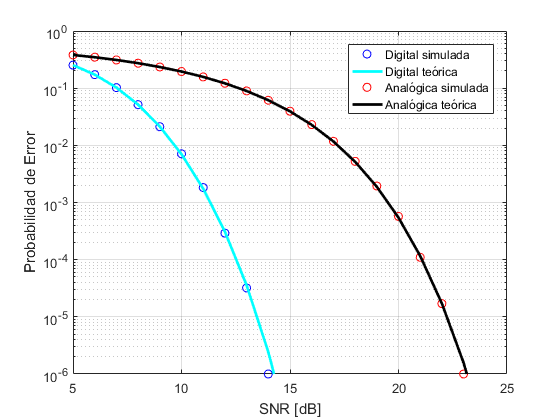
\includegraphics[width=\textwidth]{./Matlab/ej4h=1n=1meg.png}
    \caption{Probabilidad de error en función del SNR, simulada y teórica. }
\label{fig:mc_h1}
\end{figure}

Puede verse que las curvas teóricas corresponden con muy buena precisión a los puntos simulados. Esto se debe a que, al generarse una cantidad muy grande de entradas simuladas, el cociente de errores y realizaciones aproxima estadísticamente la probabilidad del error.

En particular, este gráfico se generó con un millón de realizaciones para cada sistema y valor de \textbf{SNR}; sin embargo, se observó que a partir de aproximadamente veinte mil realizaciones puede notarse una clara tendencia a aproximarse a las curvas teóricas. 

\begin{figure}[H]
	\centering
	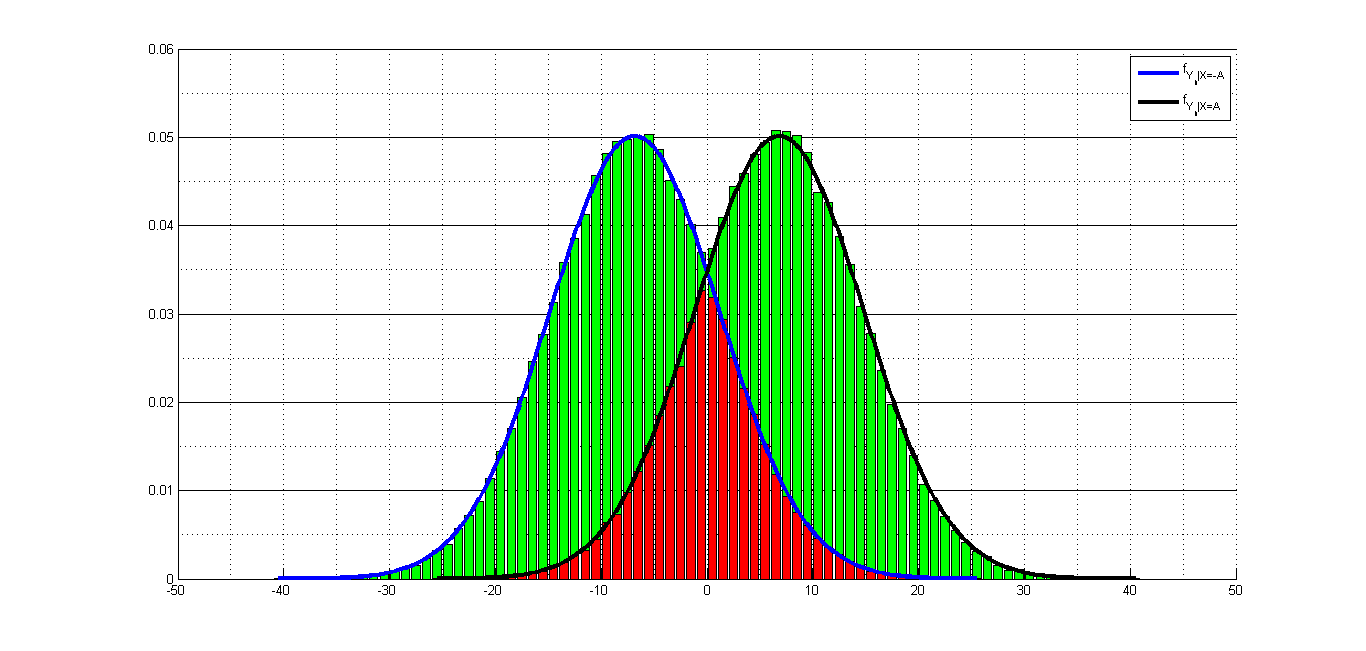
\includegraphics[width=\textwidth]{./Matlab/pdfs}
	\caption{Graficas de las densiades de probabilidad. }
	\label{fig:pdfs}
\end{figure}

Finalmente, la figura \ref{fig:pdfs} muestra las funciones de densidad de probabilidad para $Y_n|_{X_1=-A}$ y de $Y_n|_{X_1=A}$. Las mismas se encuentran superpuestas a un histograma de simulacioón, con valor arbitrario de \textbf{SNR}=10. Puede verse que se trata de un solapamiento de 2 curvas normales, tal como es de esperarse, donde la sección solapada en rojo, representa los casos de errores.